\documentclass{article}

% content/resources/templates/preamble.tex
\usepackage[margin=0.6in]{geometry}
\author{Milav Dabgar}
\usepackage{amsmath,amssymb,amsthm}
\usepackage{booktabs}
\usepackage{multirow}
\usepackage{xcolor}
\usepackage{tcolorbox}
\tcbuselibrary{breakable,skins}
\usepackage[colorlinks=true,linkcolor=blue]{hyperref}
\usepackage{titlesec}
\usepackage{enumitem}
\usepackage{tikz}
\usepackage{pgfplots}
\usepackage{circuitikz}
\usepackage[version=4]{mhchem}
\usepackage{longtable}
\usepackage{array}
\usepackage{float}
\usepackage{caption}
\usepackage{listings}

\lstset{
  basicstyle=\small\ttfamily,
  breaklines=true,
  breakatwhitespace=false,
  postbreak=\mbox{\textcolor{red}{$\hookrightarrow$}\space},
  float=false,
  numbers=left,
  numberstyle=\tiny\color{gray},
  numbersep=10pt,
  xleftmargin=2em,
  keywordstyle=\color{blue},
  commentstyle=\color{green!60!black},
  stringstyle=\color{purple},
  backgroundcolor=\color{gray!5},
  showstringspaces=false,
  tabsize=2,
  captionpos=b,
  keepspaces=true,
  columns=flexible
}

\pgfplotsset{compat=1.18}
\usetikzlibrary{shapes,arrows,positioning,calc,patterns,decorations.pathmorphing,decorations.markings,arrows.meta}

% Color scheme
\definecolor{headcolor}{RGB}{0,102,204}
\definecolor{keycolor}{RGB}{220,20,60}
\definecolor{solutioncolor}{RGB}{34,139,34}
\definecolor{mnemoniccolor}{RGB}{148,0,211}
\definecolor{codecolor}{RGB}{0,0,100}

% Spacing
\setlength{\parskip}{3pt}
\setlist[itemize]{nosep}
\setlist[enumerate]{nosep}

% Title formatting
\titleformat{\section}{\Large\bfseries\color{headcolor}}{\thesection}{1em}{}
\titleformat{\subsection}{\large\bfseries\color{headcolor}}{\thesubsection}{1em}{}

% Pandoc tightlist compatibility
\providecommand{\tightlist}{%
  \setlength{\itemsep}{0pt}\setlength{\parskip}{0pt}}

% Pandoc longtable compatibility
\newcounter{none}
\def\thenone{}


% content/resources/templates/english-boxes.tex

% Custom environments
\newtcolorbox{solutionbox}{
 breakable,
 enhanced,
 colback=solutioncolor!5!white,
 colframe=solutioncolor!75!black,
 fonttitle=\bfseries,
 title=Solution
}

\newtcolorbox{solutionboxnobreak}{
 colback=solutioncolor!5!white,
 colframe=solutioncolor!75!black,
 fonttitle=\bfseries,
 title=Solution
}

\newtcolorbox{keyformula}{
 breakable,
 enhanced,
 colback=keycolor!5!white,
 colframe=keycolor!75!black,
 fonttitle=\bfseries,
 title=Key Formula
}

\newtcolorbox{mnemonicboxenv}{
 breakable,
 enhanced,
 colback=mnemoniccolor!5!white,
 colframe=mnemoniccolor!75!black,
 fonttitle=\bfseries,
 title=Mnemonic
}

\newcommand{\mnemonicbox}[1]{%
  \begin{mnemonicboxenv}
    #1
  \end{mnemonicboxenv}
}


% Custom commands for GTU solutions
% This file defines semantic commands for consistent formatting

% Question command with automatic formatting
\newcommand{\question}[2]{%
  \section*{Question #1}%
  \textbf{#2}%
}

% OR question variant
\newcommand{\questionor}[2]{%
  \section*{Question #1 OR}%
  \textbf{#2}%
}

% Proper table environment with caption
\newenvironment{answertable}[1]{%
  \begin{table}[htbp]
  \centering
  \caption{#1}
}{%
  \end{table}
}

% Proper figure environment for diagrams
\newenvironment{answerdiagram}[1]{%
  \begin{figure}[htbp]
  \centering
  \caption{#1}
}{%
  \end{figure}
}

% Semantic markup for key terms
\newcommand{\keyword}[1]{\textbf{#1}}
\newcommand{\code}[1]{\texttt{#1}}
\newcommand{\classname}[1]{\texttt{#1}}
\newcommand{\methodname}[1]{\texttt{#1}}

% Proper quotation marks
\newcommand{\mnemonic}[1]{``#1''}


\title{Antenna and Wave Propagation (4341106) - Summer 2024 Solution}
\date{June 19, 2024}

\begin{document}
\maketitle

\questionmarks{1(a)}{3}{Define Beam Area and Beam Efficiency.}

\begin{solutionbox}
\textbf{Beam Area}: The solid angle through which all of the power radiated by an antenna would flow if the radiation intensity was constant throughout this angle and equal to the maximum value.

\textbf{Beam Efficiency}: The ratio of the power contained in the main beam to the total power radiated by the antenna.

\begin{answerdiagram}{Beam Efficiency Concept}
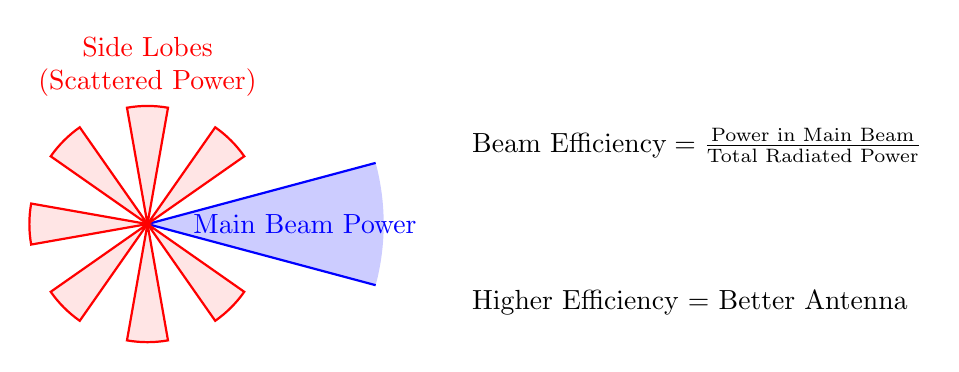
\begin{tikzpicture}
    % Main Beam
    \fill [blue!20] (0,0) -- (15:3) arc (15:-15:3) -- cycle;
    \draw [thick, blue] (0,0) -- (15:3);
    \draw [thick, blue] (0,0) -- (-15:3);
    \node [blue] at (2, 0) {Main Beam Power};
    
    % Side lobes (minor)
    \foreach \angle in {45, 90, 135, 180, 225, 270, 315} {
        \draw [thick, red, fill=red!10] (0,0) -- (\angle-10:1.5) arc (\angle-10:\angle+10:1.5) -- cycle;
    }
    \node [red, align=center] at (0, 2) {Side Lobes\\(Scattered Power)};
    
    \node [align=left, anchor=west] at (4, 1) {$\text{Beam Efficiency} = \frac{\text{Power in Main Beam}}{\text{Total Radiated Power}}$};
    \node [align=left, anchor=west] at (4, -1) {Higher Efficiency = Better Antenna};
\end{tikzpicture}
\end{answerdiagram}
\end{solutionbox}

\begin{mnemonicbox}
\mnemonic{"BEAM: Better Efficiency Achieves Maximum performance"}
\end{mnemonicbox}

\questionmarks{1(b)}{4}{What is EM field? Explain its radiation from center fed dipole.}

\begin{solutionbox}
\textbf{EM Field}: An Electromagnetic (EM) field is a physical field produced by electrically charged objects. It affects the behavior of charged objects in the vicinity of the field.

\textbf{Radiation from Center-Fed Dipole}:
When an alternating current flows through the dipole, it creates oscillating electric and magnetic fields that detach and travel outwards.

\begin{answerdiagram}{Fields around a Dipole}
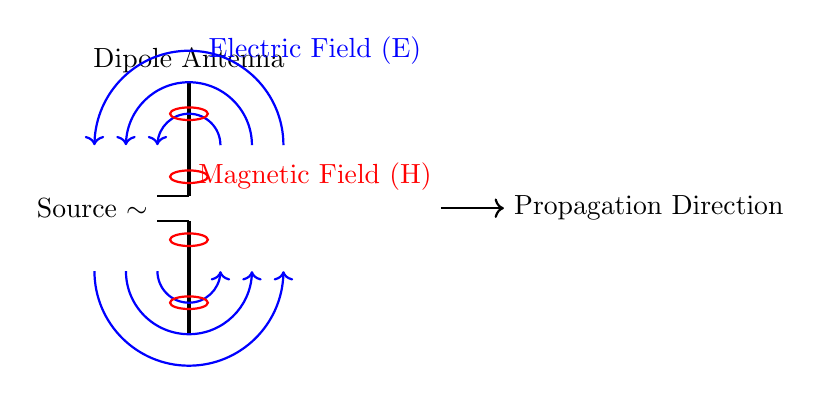
\begin{tikzpicture}[scale=0.8]
    % Dipole
    \draw [ultra thick] (0, 2) -- (0, 0.2);
    \draw [ultra thick] (0, -2) -- (0, -0.2);
    \draw [thick] (-0.5, 0.2) -- (0, 0.2);
    \draw [thick] (-0.5, -0.2) -- (0, -0.2);
    \node [left] at (-0.5, 0) {Source $\sim$};
    \node [above] at (0, 2) {Dipole Antenna};

    % E-Fields (Loops)
    \foreach \x in {1, 2, 3} {
        \draw [blue, thick, ->] (0.5*\x, 1) arc (0:180:0.5*\x) node [midway, above] {};
        \draw [blue, thick, ->] (-0.5*\x, -1) arc (180:360:0.5*\x);
    }
    \node [blue] at (2, 2.5) {Electric Field (E)};

    % H-Fields (Circles around wire)
    \foreach \y in {-1.5, -0.5, 0.5, 1.5} {
        \draw [red, thick] (0, \y) ellipse (0.3 and 0.1);
    }
    \node [red] at (2, 0.5) {Magnetic Field (H)};
    
    \draw [->, thick] (4, 0) -- (5, 0) node [right] {Propagation Direction};
\end{tikzpicture}
\end{answerdiagram}

\begin{itemize}
    \item \textbf{Electric field (E)}: Lines start from positive charge and end at negative charge.
    \item \textbf{Magnetic field (H)}: Circles around the current carrier (wire).
    \item \textbf{Mechanism}: As current reverses, field lines detach and form closed loops (radiation).
    \item \textbf{Far Field}: E and H are perpendicular to each other and to the direction of propagation.
\end{itemize}
\end{solutionbox}

\begin{mnemonicbox}
\mnemonic{"CERD: Current Excites Radiating Dipole"}
\end{mnemonicbox}

\questionmarks{1(c)}{7}{Explain Power radiated by elementary dipole using Poynting Vector.}

\begin{solutionbox}
Power radiated by an elementary dipole is calculated using the Poynting vector, which represents directional energy flux density.

\begin{center}
\begin{tikzpicture}[node distance=1.5cm, auto]
    \node [gtu block] (step1) {1. Calculate E-field ($E_\theta, E_\phi$)};
    \node [gtu block, below=of step1] (step2) {2. Calculate H-field ($H_\theta, H_\phi$)};
    \node [gtu block, below=of step2] (step3) {3. Poynting Vector $P = E \times H^*$};
    \node [gtu block, below=of step3] (step4) {4. Integrate over Sphere Surface};
    \node [gtu block, below=of step4] (result) {Result: $P_{rad} = 80\pi^2 I^2 (l/\lambda)^2$};

    \draw [gtu arrow] (step1) -- (step2);
    \draw [gtu arrow] (step2) -- (step3);
    \draw [gtu arrow] (step3) -- (step4);
    \draw [gtu arrow] (step4) -- (result);
\end{tikzpicture}
\end{center}

\textbf{Key Steps:}
\begin{enumerate}
    \item \textbf{Fields}:
    $$E_\theta = j\frac{\eta I_0 dl}{2\lambda r} \sin\theta e^{-j\beta r}$$
    $$H_\phi = j\frac{I_0 dl}{2\lambda r} \sin\theta e^{-j\beta r}$$
    
    \item \textbf{Poynting Vector Magnitude} ($P_{avg}$):
    $$P_{avg} = \frac{1}{2} Re(E \times H^*) = \frac{1}{2} \frac{\eta |I_0|^2 (dl)^2}{4\lambda^2 r^2} \sin^2\theta$$
    
    \item \textbf{Total Radiated Power} ($P_{rad}$):
    Integrate $P_{avg}$ over a closed sphere surface ($ds = r^2 \sin\theta d\theta d\phi$):
    $$P_{rad} = \int_{0}^{2\pi} \int_{0}^{\pi} P_{avg} r^2 \sin\theta d\theta d\phi$$
    $$P_{rad} = \eta \frac{\pi}{3} \left(\frac{I_0 dl}{\lambda}\right)^2$$
    Using $\eta = 120\pi \approx 377 \Omega$:
    $$P_{rad} = 80\pi^2 I_{rms}^2 \left(\frac{dl}{\lambda}\right)^2 \text{ Watts}$$
\end{enumerate}
\end{solutionbox}

\begin{mnemonicbox}
\mnemonic{"PEHP: Poynting Explains How Power propagates"}
\end{mnemonicbox}

\orquestionmarks{1(c)}{7}{Define Antenna, Radiation Pattern, Directivity, Gain, FBR, Isotropic Radiator and Effective Aperture.}

\begin{solutionbox}
\begin{tabulary}{\linewidth}{|L|L|}
\hline
\textbf{Parameter} & \textbf{Definition} \\ \hline
\keyword{Antenna} & A device that converts guided electromagnetic waves to free-space waves and vice versa. \\ \hline
\keyword{Radiation Pattern} & A graphical representation of the radiation properties of the antenna as a function of space coordinates. \\ \hline
\keyword{Directivity} & The ratio of radiation intensity in a given direction to the average radiation intensity. \\ \hline
\keyword{Gain} & The ratio of radiation intensity in a given direction to the radiation intensity that would be obtained if the power accepted by the antenna were radiated isotropically. Takes efficiency into account. \\ \hline
\keyword{FBR (Front-to-Back Ratio)} & The ratio of power radiated in the forward direction (main lobe) to the power radiated in the backward direction. \\ \hline
\keyword{Isotropic Radiator} & A theoretical antenna that radiates electromagnetic energy equally well in all directions. \\ \hline
\keyword{Effective Aperture} & The ratio of the power delivered to the load to the incident power density. Measures how effective an antenna is at receiving power. \\ \hline
\end{tabulary}

\begin{answerdiagram}{Antenna Parameters Overview}
\begin{tikzpicture}
    \pie[text=legend, radius=2]{
     25/Directivity,
     25/Gain,
     20/Effective Aperture,
     15/Radiation Pattern,
     15/FBR
    }
\end{tikzpicture}
\end{answerdiagram}
\end{solutionbox}

\begin{mnemonicbox}
\mnemonic{"DIAGRAM: Directivity Improves Antenna Gain, Radiation And More"}
\end{mnemonicbox}

\questionmarks{2(a)}{3}{Explain principle of pattern multiplication.}

\begin{solutionbox}
\textbf{Principle of Pattern Multiplication}:
The total field pattern of an array of non-isotropic identical point sources is the product of the individual element pattern and the array factor of the isotropic point sources.

$$ \text{Total Pattern} = \text{Element Pattern} \times \text{Array Factor} $$

\begin{answerdiagram}{Pattern Multiplication}
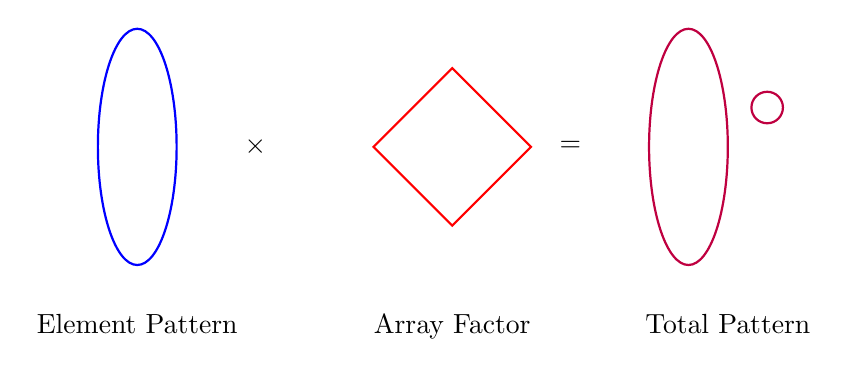
\begin{tikzpicture}
    % Element Pattern
    \draw [thick, blue] (0,0) ellipse (0.5 and 1.5);
    \node [below] at (0, -2) {Element Pattern};
    \node at (1.5, 0) {$\times$};
    
    % Array Factor
    \draw [thick, red] (3,0) -- (4, 1) -- (5,0) -- (4, -1) -- cycle; % Rough shape
    \node [below] at (4, -2) {Array Factor};
    \node at (5.5, 0) {$=$};
    
    % Result
    \draw [thick, purple] (7,0) ellipse (0.5 and 1.5); % Combined effect visual
    \draw [thick, purple] (8,0.5) circle (0.2); 
    \node [below] at (7.5, -2) {Total Pattern};
\end{tikzpicture}
\end{answerdiagram}

It helps in designing arrays with sharper beams and higher directivity without analyzing the complex geometry from scratch.
\end{solutionbox}

\begin{mnemonicbox}
\mnemonic{"PEAM: Pattern Equals Array times Element Method"}
\end{mnemonicbox}

\questionmarks{2(b)}{4}{Draw \& Explain Loop antenna.}

\begin{solutionbox}
A loop antenna is a radio antenna consisting of a loop or coil of wire, tubing, or other electrical conductor.

\begin{answerdiagram}{Loop Antenna Structure}
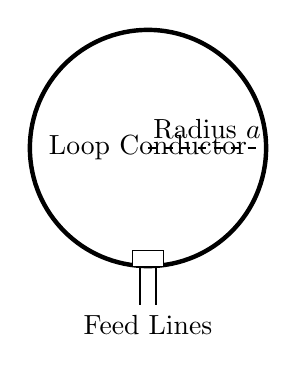
\begin{tikzpicture}
    \draw [ultra thick] (0,0) circle (1.5); % Loop
    \draw [fill=white] (-0.2, -1.5) rectangle (0.2, -1.3); % Feed gap
    \draw [thick] (-0.1, -1.5) -- (-0.1, -2);
    \draw [thick] (0.1, -1.5) -- (0.1, -2);
    \node [below] at (0, -2) {Feed Lines};
    \node at (0, 0) {Loop Conductor};
    
    % Dimensions
    \draw [dashed] (0,0) -- (1.5, 0);
    \node [above] at (0.75, 0) {Radius $a$};
\end{tikzpicture}
\end{answerdiagram}

\begin{itemize}
    \item \textbf{Small Loop} ($C < \lambda/10$): Radiation pattern similar to a magnetic dipole (Figure-8 pattern). Low radiation resistance.
    \item \textbf{Large Loop} ($C \approx \lambda$): Resonant loop. Maximum radiation perpendicular to the loop plane.
    \item \textbf{Applications}: Direction finding (RDF), AM radio reception, RFID tags.
\end{itemize}
\end{solutionbox}

\begin{mnemonicbox}
\mnemonic{"LOOP: Low Output, Orientation Precise"}
\end{mnemonicbox}

\questionmarks{2(c)}{7}{Design a Yagi-uda antenna and explain it.}

\begin{solutionbox}
A Yagi-Uda antenna is a directional antenna consisting of a driven element (usually a dipole) and additional parasitic elements (reflector and directors).

\textbf{Design Guidelines:}
\begin{tabulary}{\linewidth}{|L|L|L|}
\hline
\textbf{Element} & \textbf{Length Formula} & \textbf{Typical Spacing} \\ \hline
Reflector & $0.5\lambda \times 1.05$ (approx $0.525\lambda$) & $0.15\lambda - 0.25\lambda$ from Driven \\ \hline
Driven Element & $0.5\lambda$ (resonant length) & Reference (0) \\ \hline
Director 1 & $0.5\lambda \times 0.95$ & $0.1\lambda - 0.15\lambda$ from Driven \\ \hline
Director 2 & $0.5\lambda \times 0.92$ & $0.15\lambda - 0.25\lambda$ from D1 \\ \hline
\end{tabulary}

\begin{answerdiagram}{Yagi-Uda Antenna Structure}
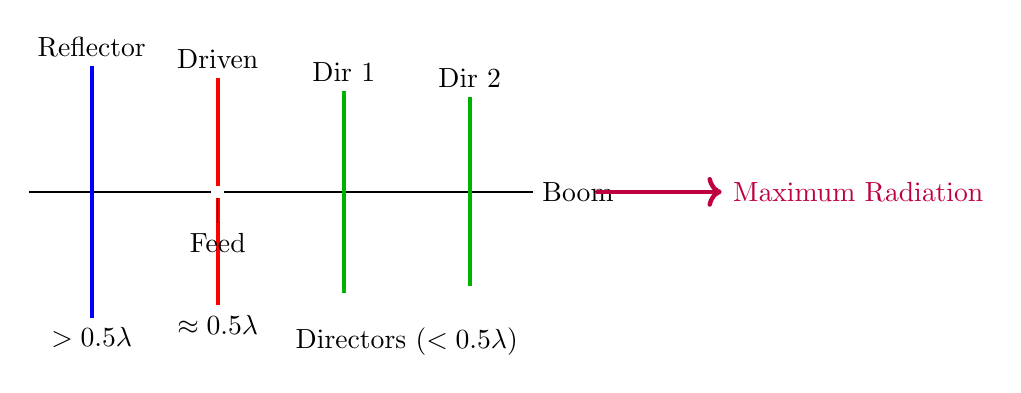
\begin{tikzpicture}[scale=0.8]
    % Boom
    \draw [thick] (-2, 0) -- (6, 0);
    \node [right] at (6, 0) {Boom};
    
    % Reflector
    \draw [ultra thick, blue] (-1, -2) -- (-1, 2);
    \node [above] at (-1, 2) {Reflector};
    \node [below] at (-1, -2) {$>0.5\lambda$};
    
    % Driven Element
    \draw [ultra thick, red] (1, -1.8) -- (1, 1.8);
    \node [above] at (1, 1.8) {Driven};
    \node [below] at (1, -1.8) {$\approx 0.5\lambda$};
    \fill [white] (0.9, -0.1) rectangle (1.1, 0.1); % Feed point
    \draw (1, -0.1) -- (1, -0.5) node [below] {Feed};
    
    % Directors
    \draw [ultra thick, green!70!black] (3, -1.6) -- (3, 1.6);
    \node [above] at (3, 1.6) {Dir 1};
    
    \draw [ultra thick, green!70!black] (5, -1.5) -- (5, 1.5);
    \node [above] at (5, 1.5) {Dir 2};
    \node [below] at (4, -2) {Directors ($<0.5\lambda$)};
    
    % Radiation
    \draw [->, ultra thick, purple] (7, 0) -- (9, 0) node [right] {Maximum Radiation};
\end{tikzpicture}
\end{answerdiagram}

\begin{itemize}
    \item \textbf{Reflector}: Longer than driven element, reflects energy forward.
    \item \textbf{Directors}: Shorter than driven element, guide energy forward.
    \item \textbf{Gain}: High gain (10-20 dB depending on elements).
    \item \textbf{Impedance}: Low input impedance (20-50$\Omega$), often requires a balun.
    \item \textbf{Application}: TV reception, amateur radio, point-to-point links.
\end{itemize}
\end{solutionbox}

\begin{mnemonicbox}
\mnemonic{"YARD: Yagi Achieves Radical Directivity"}
\end{mnemonicbox}

\orquestionmarks{2(a)}{3}{Compare broad fire and end fire array antenna.}

\begin{solutionbox}
\begin{tabulary}{\linewidth}{|L|L|L|}
\hline
\textbf{Parameter} & \textbf{Broadside Array} & \textbf{End Fire Array} \\ \hline
\keyword{Direction of Max Radiation} & Perpendicular to the array axis. & Along the array axis. \\ \hline
\keyword{Element Phasing} & All elements fed in phase (0$^\circ$). & Progressive phase shift ($\approx 180^\circ$). \\ \hline
\keyword{Beamwidth} & Narrower main beam. & Wider main beam. \\ \hline
\keyword{Directivity} & Generally higher for same length. & Lower than broadside. \\ \hline
\keyword{Applications} & Broadcasting arrays. & Point-to-point links. \\ \hline
\end{tabulary}

\begin{answerdiagram}{Array Comparison}
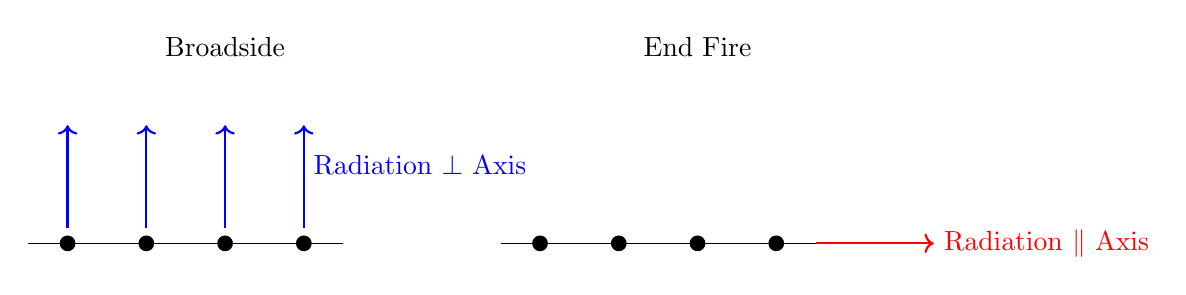
\begin{tikzpicture}
    % Broadside
    \node [align=center] at (2, 2.5) {Broadside};
    \foreach \x in {0, 1, 2, 3} \fill (\x, 0) circle (0.1);
    \draw (-0.5, 0) -- (3.5, 0);
    \foreach \x in {0, 1, 2, 3} \draw [->, thick, blue] (\x, 0.2) -- (\x, 1.5);
    \node [right, blue] at (3, 1) {Radiation $\perp$ Axis};

    % End Fire
    \node [align=center] at (8, 2.5) {End Fire};
    \foreach \x in {6, 7, 8, 9} \fill (\x, 0) circle (0.1);
    \draw (5.5, 0) -- (9.5, 0);
    \draw [->, thick, red] (9.5, 0) -- (11, 0) node [right] {Radiation $\parallel$ Axis};
\end{tikzpicture}
\end{answerdiagram}
\end{solutionbox}

\begin{mnemonicbox}
\mnemonic{"BEPS: Broadside Emits Perpendicularly, Sideways"}
\end{mnemonicbox}

\orquestionmarks{2(b)}{4}{Draw \& Explain Folded dipole antenna.}

\begin{solutionbox}
A folded dipole consists of two parallel dipoles connected at both ends, forming a narrow loop. One side is fed at the center.

\begin{answerdiagram}{Folded Dipole}
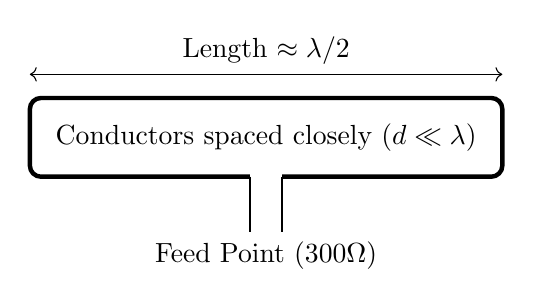
\begin{tikzpicture}
    \draw [ultra thick, rounded corners] (-3, 0.5) rectangle (3, -0.5);
    \fill [white] (-0.2, -0.6) rectangle (0.2, -0.4); % Break
    \draw [thick] (-0.2, -0.5) -- (-0.2, -1.2);
    \draw [thick] (0.2, -0.5) -- (0.2, -1.2);
    \node [below] at (0, -1.2) {Feed Point (300$\Omega$)};
    
    \draw [<->] (-3, 0.8) -- (3, 0.8) node [midway, above] {Length $\approx \lambda/2$};
    \node at (0, 0) {Conductors spaced closely ($d \ll \lambda$)};
\end{tikzpicture}
\end{answerdiagram}

\begin{itemize}
    \item \textbf{Input Impedance}: Approx 300$\Omega$ (4 times that of a standard dipole's 73$\Omega$).
    \item \textbf{Bandwidth}: Much wider bandwidth than a simple dipole.
    \item \textbf{Applications}: Standard FM radio antennas, TV reception (uses 300$\Omega$ twin-lead cable).
    \item \textbf{Advantage}: Acts as a step-up impedance transformer.
\end{itemize}
\end{solutionbox}

\begin{mnemonicbox}
\mnemonic{"FIBER: Folded Impedance Booster Enhances Reception"}
\end{mnemonicbox}

\orquestionmarks{2(c)}{7}{Give names of Non-resonant antennas and explain any one in detail with its radiation pattern.}

\begin{solutionbox}
\textbf{Non-Resonant Antennas}:
1. Rhombic Antenna
2. V-Antenna
3. Beverage Antenna (Wave antenna)
4. Long Wire Antenna

\textbf{Rhombic Antenna Explanation}:
A Rhombic antenna consists of four long wire conductors arranged in a diamond (rhombus) shape. It is a traveling wave antenna terminated in a load resistance $R$ to remove reflection.

\begin{answerdiagram}{Rhombic Antenna}
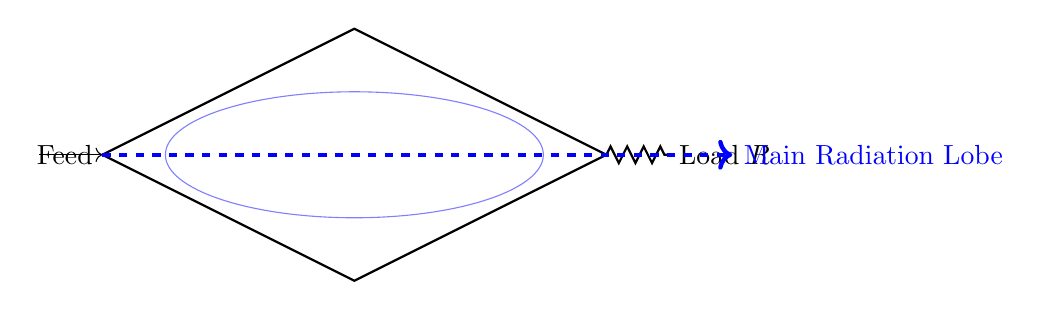
\begin{tikzpicture}[scale=0.8]
    \coordinate (Feed) at (0,0);
    \coordinate (Top) at (4, 2);
    \coordinate (Bottom) at (4, -2);
    \coordinate (Load) at (8, 0);

    \draw [thick] (Feed) -- (Top) -- (Load);
    \draw [thick] (Feed) -- (Bottom) -- (Load);
    
    \draw [->] (-1, 0) -- (0, 0) node [left] {Feed};
    \draw [thick, decorate, decoration={zigzag, amplitude=3pt, segment length=6pt}] (Load) -- (9, 0);
    \node [right] at (9, 0) {Load $R$};
    
    \draw [->, ultra thick, dashed, blue] (0, 0) -- (10, 0) node [right] {Main Radiation Lobe};
    
    % Side lobes hint
    \draw [blue, opacity=0.5] (4,0) ellipse (3 and 1); 
\end{tikzpicture}
\end{answerdiagram}

\textbf{Characteristics}:
\begin{itemize}
    \item \textbf{Structure}: Non-resonant due to resistive termination.
    \item \textbf{Radiation Pattern}: Unidirectional (due to termination). Without R, it would be bidirectional.
    \item \textbf{Gain}: High gain (up to 15-20 dB).
    \item \textbf{Bandwidth}: Very wide bandwidth.
    \item \textbf{Applications}: HF point-to-point communication.
\end{itemize}
\end{solutionbox}

\begin{mnemonicbox}
\mnemonic{"RHOMBIC: Reliable High-Output Multi-Band Impressive Communications"}
\end{mnemonicbox}

\questionmarks{3(a)}{3}{Compare radiation pattern of different resonant wire antennas.}

\begin{solutionbox}
\begin{tabulary}{\linewidth}{|L|L|L|L|}
\hline
\textbf{Antenna Type} & \textbf{Pattern Shape} & \textbf{Directivity} & \textbf{Polarization} \\ \hline
Half-Wave Dipole ($\lambda/2$) & Figure-8 (donut shape), 2 lobes & 2.15 dBi & Linear \\ \hline
Full-Wave Dipole ($\lambda$) & Four-lobed (cloverleaf) & 3.8 dBi & Linear \\ \hline
$3\lambda/2$ Dipole & Six-lobed & 4.2 dBi & Linear \\ \hline
$2\lambda$ Dipole & Eight-lobed & 4.5 dBi & Linear \\ \hline
\end{tabulary}

\begin{answerdiagram}{Resonant Antenna Patterns}
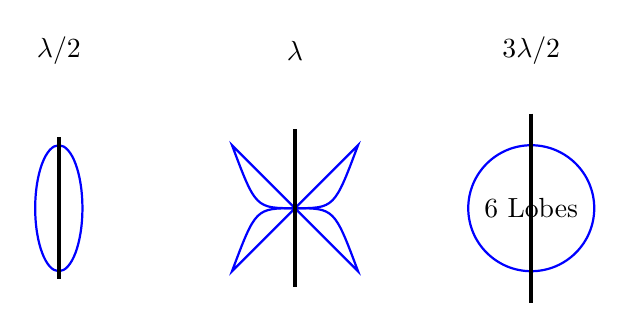
\begin{tikzpicture}
    % Half Wave
    \node at (0, 2) {$\lambda/2$};
    \draw [thick, blue] (0, 0) ellipse (0.3 and 0.8);
    \draw [ultra thick] (0, 0.9) -- (0, -0.9); % Antenna
    
    % Full Wave
    \node at (3, 2) {$\lambda$};
    \draw [thick, blue] (3, 0) .. controls (3.5, 0.5) .. (3.8, 0.8) .. controls (3.5, 0) .. (3,0);
    \draw [thick, blue] (3, 0) .. controls (2.5, 0.5) .. (2.2, 0.8) .. controls (2.5, 0) .. (3,0);
    \draw [thick, blue] (3, 0) .. controls (3.5, -0.5) .. (3.8, -0.8) .. controls (3.5, 0) .. (3,0);
    \draw [thick, blue] (3, 0) .. controls (2.5, -0.5) .. (2.2, -0.8) .. controls (2.5, 0) .. (3,0);
    \draw [ultra thick] (3, 1) -- (3, -1);

    % 3/2 Lambda (Simplified)
    \node at (6, 2) {$3\lambda/2$};
    \draw [thick, blue] (6,0) circle (0.8); \node at (6,0) {6 Lobes};
    \draw [ultra thick] (6, 1.2) -- (6, -1.2);
\end{tikzpicture}
\end{answerdiagram}
\end{solutionbox}

\begin{mnemonicbox}
\mnemonic{"MOLD: More wavelengths create Lots of Directivity lobes"}
\end{mnemonicbox}

\questionmarks{3(b)}{4}{Draw V and Inverted V antenna with radiation Pattern.}

\begin{solutionbox}
\begin{answerdiagram}{V and Inverted-V Antennas}
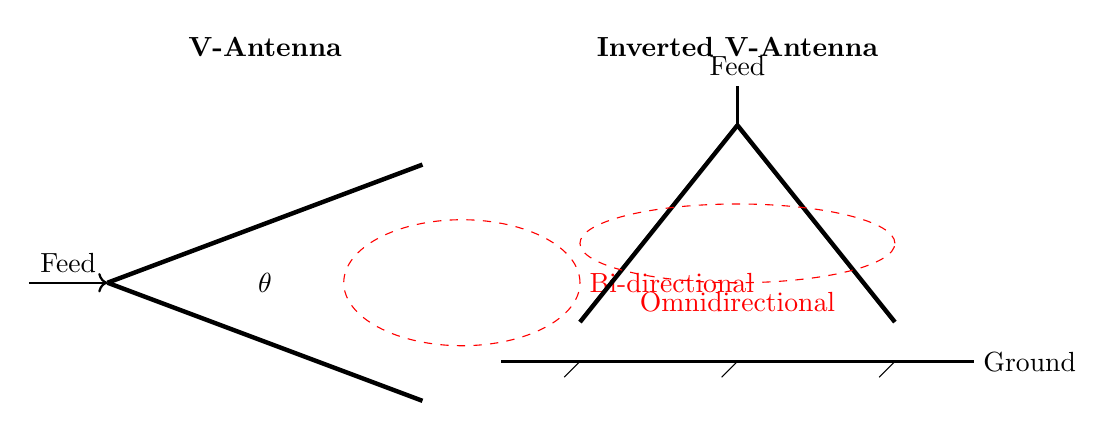
\begin{tikzpicture}
    % V Antenna
    \node [font=\bfseries] at (2, 3) {V-Antenna};
    \draw [ultra thick] (0, 0) -- (4, 1.5);
    \draw [ultra thick] (0, 0) -- (4, -1.5);
    \draw [thick, ->] (-1, 0) -- (0, 0) node [midway, above] {Feed};
    \draw [dashed, red] (4.5, 0) ellipse (1.5 and 0.8);
    \node [red, right] at (6, 0) {Bi-directional};
    \node at (2, 0) {$\theta$};

    % Inverted V
    \node [font=\bfseries] at (8, 3) {Inverted V-Antenna};
    \draw [ultra thick] (8, 2) -- (6, -0.5);
    \draw [ultra thick] (8, 2) -- (10, -0.5);
    \draw [thick] (8, 2) -- (8, 2.5) node [above] {Feed};
    \draw [thick] (5, -1) -- (11, -1); \node [right] at (11, -1) {Ground};
    \foreach \x in {6, 8, 10} \draw (\x, -1) -- (\x-0.2, -1.2);
    
    \draw [dashed, red] (8, 0.5) ellipse (2 and 0.5);
    \node [red, below] at (8, 0) {Omnidirectional};
\end{tikzpicture}
\end{answerdiagram}

\begin{itemize}
    \item \textbf{V-Antenna}: Two wires forming a V-shape. Main radiation is along the axis of the V (if resonant).
    \item \textbf{Inverted V}: A dipole supported at the center with ends drooping. Pattern is nearly omnidirectional.
\end{itemize}
\end{solutionbox}

\begin{mnemonicbox}
\mnemonic{"VIPS: V-shapes Improve Pattern Selectivity"}
\end{mnemonicbox}

\questionmarks{3(c)}{7}{Explain Morse Code and Practice Oscillator.}

\begin{solutionbox}
\textbf{Morse Code}: A character encoding scheme used in telecommunication that encodes text characters as standardized sequences of two different signal durations, called dots and dashes.

\begin{tabulary}{\linewidth}{|L|L|L|}
\hline
\textbf{Element} & \textbf{Timing} & \textbf{Sound} \\ \hline
Dot (.) & 1 Unit & Short Beep \\ \hline
Dash (-) & 3 Units & Long Beep \\ \hline
Inter-element space & 1 Unit & Silence \\ \hline
Character space & 3 Units & Silence \\ \hline
Word space & 7 Units & Silence \\ \hline
\end{tabulary}

\begin{answerdiagram}{Morse Code Practice Oscillator using 555 Timer}
\begin{tikzpicture}[circuit ee IEC, set resistor graphic=var resistor IEC graphic]
    \node [draw, rectangle, minimum width=2cm, minimum height=2.5cm, align=center] (IC) at (0,0) {555\\Timer};
    
    % Power
    \draw (IC.north) -- ++(0, 1) node [above] {+9V};
    
    % Speaker Output (Pin 3)
    \draw (IC.east) -- ++(1, 0) to [loudspeaker] ++(1, 0) -- ++(0, -2) coordinate (GND);
    
    % Key and Ground (Pin 1)
    \draw (IC.south) -- ++(0, -0.5) to [make contact={info={Key}}] ++(0, -1) -- (0, -2) node [ground] {};
    
    % Timing Components
    \draw (-2, 1) -- (0, 1); % Vcc rail
    \draw (-2, 1) to [resistor={info={$R_1$}}] (-2, 0) -- (IC.west);
    \draw (-2, 0) to [resistor={info={$R_2$}}] (-2, -1.5) to [capacitor={info={$C_1$}}] (-2, -2) -- (0, -2);
\end{tikzpicture}
\end{answerdiagram}

\textbf{Operation}:
The 555 timer is configured as an astable multivibrator. When the key is pressed, the circuit is completed, creating an audio tone (600-800 Hz) driving the speaker.
\end{solutionbox}

\begin{mnemonicbox}
\mnemonic{"TEMPO: Timing Elements Make Perfect Oscillation"}
\end{mnemonicbox}

\orquestionmarks{3(a)}{3}{Draw and Explain Microstrip Patch antenna.}

\begin{solutionbox}
A Microstrip Patch Antenna consists of a radiating patch on one side of a dielectric substrate and a ground plane on the other side.

\begin{answerdiagram}{Microstrip Patch Antenna}
\begin{tikzpicture}
    % Ground Plane
    \fill [gray!20] (0,0) rectangle (6,4);
    \draw [thick] (0,0) rectangle (6,4);
    \node [below] at (3,0) {Ground Plane (Bottom)};

    % Substrate (implied thickness)
    \draw [dashed] (0.5, 0.5) rectangle (5.5, 3.5);
    \node at (5, 3) {Substrate $\epsilon_r$};

    % Patch
    \fill [orange!40] (1.5, 1) rectangle (4.5, 3);
    \draw [thick] (1.5, 1) rectangle (4.5, 3);
    \node at (3, 2) {Radiating Patch (Metal)};

    % Feed Line
    \draw [thick, fill=orange!40] (3, 1) -- (3, 0) -- (3.2, 0) -- (3.2, 1);
    \node [below right] at (3.2, 0.5) {Microstrip Feed};
    
    % Radiation
    \foreach \x in {1.5, 4.5} \draw [->, red, snake=coil, segment aspect=0] (\x, 3.2) -- (\x, 4.2);
    \node [red, above] at (3, 4.2) {Fringing Fields (Radiation)};
\end{tikzpicture}
\end{answerdiagram}

\begin{itemize}
    \item \textbf{Advantages}: Low profile, lightweight, easy to fabricate, conformable to surfaces.
    \item \textbf{Disadvantages}: Narrow bandwidth, low efficiency.
    \item \textbf{Applications}: Mobile phones, GPS, aircraft, satellites.
\end{itemize}
\end{solutionbox}

\begin{mnemonicbox}
\mnemonic{"MAPS: Microstrip Antenna Patches are Simple"}
\end{mnemonicbox}

\orquestionmarks{3(b)}{4}{Draw and Explain Horn antenna.}

\begin{solutionbox}
A Horn Antenna is a waveguide flared out at the end to improve radiation efficiency and directivity.

\begin{answerdiagram}{Horn Antenna}
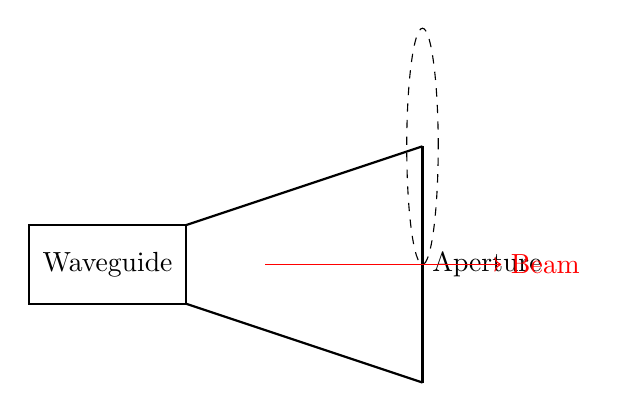
\begin{tikzpicture}
    % Waveguide section
    \draw [thick] (0, 0.5) rectangle (2, 1.5);
    \node at (1, 1) {Waveguide};
    
    % Flared Horn
    \draw [thick] (2, 1.5) -- (5, 2.5);
    \draw [thick] (2, 0.5) -- (5, -0.5);
    \draw [thick] (5, 2.5) -- (5, -0.5); % Aperture
    \draw [dashed] (5, 2.5) ellipse (0.2 and 1.5);
    
    % Labels
    \node [right] at (5, 1) {Aperture};
    \draw [->, red] (3, 1) -- (6, 1) node [right] {Beam};
\end{tikzpicture}
\end{answerdiagram}

\begin{itemize}
    \item \textbf{Function}: Acts as an impedance matching transformer between the waveguide (impedance $\approx$ characteristic Z) and free space (377$\Omega$).
    \item \textbf{Types}: Sectoral E-plane, Sectoral H-plane, Pyramidal, Conical.
    \item \textbf{Applications}: Standard gain reference, feed for parabolic dishes.
\end{itemize}
\end{solutionbox}

\begin{mnemonicbox}
\mnemonic{"HEWB: Horns Enhance Waveguide Beamwidth"}
\end{mnemonicbox}

\orquestionmarks{3(c)}{7}{List different feed system for Parabolic reflector antenna and explain any one.}

\begin{solutionbox}
\textbf{Feed Systems}:
1. Front Feed (Primary Feed)
2. Cassegrain Feed
3. Gregorian Feed
4. Offset Feed

\textbf{Front Feed System Explanation}:
The primary radiator (feed antenna, usually a horn) is placed at the focal point of the parabolic reflector.

\begin{answerdiagram}{Front Feed Parabolic Reflector}
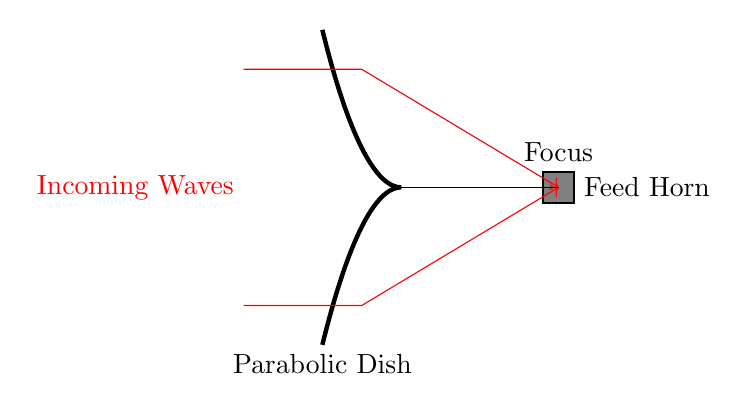
\begin{tikzpicture}
    % Parabola
    \draw [ultra thick] (0, -2) parabola bend (1, 0) (0, 2);
    \node [below] at (0, -2) {Parabolic Dish};

    % Focus and Feed
    \fill (3, 0) circle (0.1);
    \node [above] at (3, 0.2) {Focus};
    \draw [thick, fill=gray] (2.8, -0.2) rectangle (3.2, 0.2);
    \node [right] at (3.2, 0) {Feed Horn};
    
    % Rays
    \draw [->, red] (-1, 1.5) -- (0.5, 1.5) -- (3, 0);
    \draw [->, red] (-1, -1.5) -- (0.5, -1.5) -- (3, 0);
    \node [red, left] at (-1, 0) {Incoming Waves};
    
    % Support
    \draw [thin] (1, 0) -- (3, 0);
\end{tikzpicture}
\end{answerdiagram}

\begin{itemize}
    \item \textbf{Operation}: The parabolic shape reflects incoming parallel rays to a single focal point where the feed collects them. In transmission, the feed radiates to the reflector, which collimates the beam.
    \item \textbf{Advantages}: Simple construction.
    \item \textbf{Disadvantages}: Aperture blockage by feed and supports reduces efficiency.
\end{itemize}
\end{solutionbox}

\begin{mnemonicbox}
\mnemonic{"FACTS: Focused Aperture Captures Transmitted Signals"}
\end{mnemonicbox}

\questionmarks{4(a)}{3}{Explain working principle of HAM radio.}

\begin{solutionbox}
HAM radio (Amateur Radio) is a popular hobby and service that brings people, electronics, and communication together.

\begin{answerdiagram}{HAM Radio Communication System}
\begin{tikzpicture}[node distance=2cm, auto]
    \node [gtu block] (tx) {Transmitter};
    \node [gtu block, right=of tx] (ant1) {Antenna};
    \node [cloud, draw, aspect=2, red, right=of ant1] (med) {Ionosphere};
    \node [gtu block, right=of med] (ant2) {Antenna};
    \node [gtu block, right=of ant2] (rx) {Receiver};

    \draw [gtu arrow] (tx) -- (ant1);
    \draw [gtu arrow, dashed] (ant1) -- node[above] {Radio Waves} (med);
    \draw [gtu arrow, dashed] (med) -- (ant2);
    \draw [gtu arrow] (ant2) -- (rx);
\end{tikzpicture}
\end{answerdiagram}

\begin{itemize}
    \item \textbf{Principle}: Users communicate over radio frequencies allocated by regulatory bodies (like WPC in India, FCC in US).
    \item \textbf{Modes}: Voice (AM/FM/SSB), Text (Morse Code), Digital (Packet Radio).
    \item \textbf{Key Feature}: Non-commercial exchange of messages, wireless experimentation, self-training, and emergency communication.
\end{itemize}
\end{solutionbox}

\begin{mnemonicbox}
\mnemonic{"TEAM: Transmission Enables Amateur Messages"}
\end{mnemonicbox}

\questionmarks{4(b)}{4}{Explain Duct Propagation.}

\begin{solutionbox}
Duct propagation is a phenomenon where radio signals are trapped between two layers of the atmosphere or between a layer and the ground, traveling much further than normal line-of-sight.

\begin{answerdiagram}{Atmospheric Ducting}
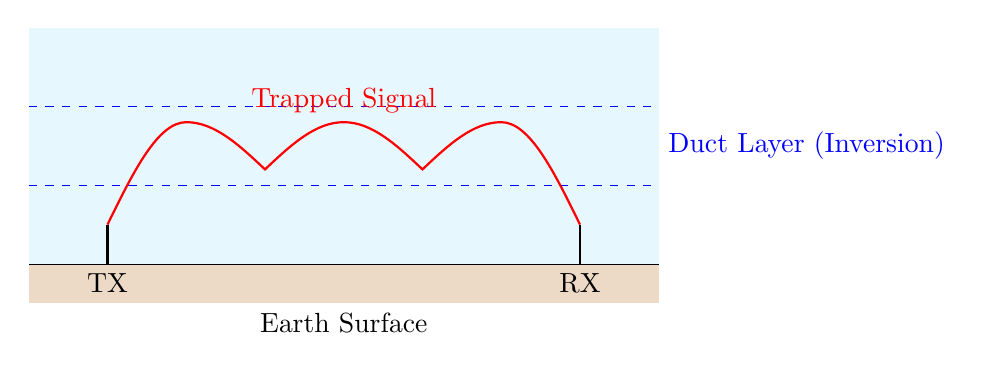
\begin{tikzpicture}
    % Ground
    \fill [brown!30] (0,0) rectangle (8, -0.5);
    \draw [thick] (0,0) -- (8,0);
    \node [below] at (4, -0.5) {Earth Surface};

    % Atmosphere Layers
    \fill [cyan!10] (0,0) rectangle (8, 3);
    \draw [dashed, blue] (0, 2) -- (8, 2);
    \draw [dashed, blue] (0, 1) -- (8, 1);
    \node [right, blue] at (8, 1.5) {Duct Layer (Inversion)};

    % Wave
    \draw [thick, red] (1, 0.5) sin (2, 1.8) cos (3, 1.2) sin (4, 1.8) cos (5, 1.2) sin (6, 1.8) cos (7, 0.5);
    \node [above, red] at (4, 1.8) {Trapped Signal};
    
    % TX/RX
    \draw [thick] (1, 0) -- (1, 0.5); \node [below] at (1,0) {TX};
    \draw [thick] (7, 0) -- (7, 0.5); \node [below] at (7,0) {RX};
\end{tikzpicture}
\end{answerdiagram}
\end{solutionbox}

\begin{mnemonicbox}
\mnemonic{"TRIP: Trapped Rays In atmospheric Paths"}
\end{mnemonicbox}

\questionmarks{4(c)}{7}{Explain Tropospheric Scattered Propagation in detail.}

\begin{solutionbox}
Tropospheric Scatter (Troposcatter) is a method of communicating with microwave radio signals over considerable distances (often up to 300 km or more) by exploiting the scattering properties of the troposphere.

\begin{answerdiagram}{Tropospheric Scatter Geometry}
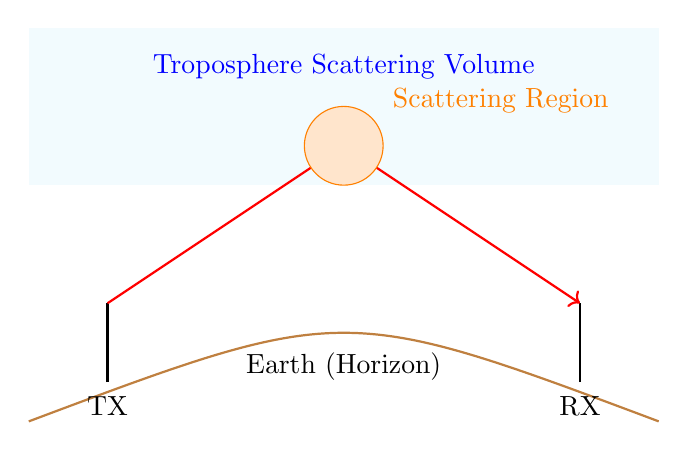
\begin{tikzpicture}
    % Earth Curve
    \draw [brown, thick] (-4, -1) .. controls (0, 0.5) .. (4, -1);
    \node [below] at (0, 0) {Earth (Horizon)};

    % Troposphere
    \fill [cyan!5] (-4, 2) rectangle (4, 4);
    \node [blue] at (0, 3.5) {Troposphere Scattering Volume};

    % TX
    \draw [thick] (-3, -0.5) -- (-3, 0.5);
    \node [black] at (-3, -0.8) {TX};
    \draw [->, red, thick] (-3, 0.5) -- (0, 2.5);
    
    % RX
    \draw [thick] (3, -0.5) -- (3, 0.5);
    \node [black] at (3, -0.8) {RX};
    \draw [<-, red, thick] (3, 0.5) -- (0, 2.5);
    
    % Scattering
    \draw [orange, fill=orange!20] (0, 2.5) circle (0.5);
    \node [above right, orange] at (0.5, 2.8) {Scattering Region};
\end{tikzpicture}
\end{answerdiagram}

\textbf{Mechanism & Characteristics}:
\begin{tabulary}{\linewidth}{|L|L|}
\hline
\textbf{Feature} & \textbf{Description} \\ \hline
\keyword{Principle} & Forward scattering due to turbulence, irregularities in refractive index, or dust/particles in the troposphere (lower atmosphere). \\ \hline
\keyword{Frequency} & Typically UHF and SHF (300 MHz - 10 GHz). \\ \hline
\keyword{Region} & Common Scattering Volume: The intersection of the transmit and receive antenna beams. \\ \hline
\keyword{Requirements} & High gain antennas and high power transmitters are needed due to high path loss. \\ \hline
\keyword{Reliability} & Fairly reliable, unaffected by ionospheric disturbances, but subject to fading. \\ \hline
\end{tabulary}
\end{solutionbox}

\begin{mnemonicbox}
\mnemonic{"STARS: Scatter Tropospheric Allows Range beyond Sight"}
\end{mnemonicbox}

\orquestionmarks{4(a)}{3}{Draw turnstile and super turnstile antenna.}

\begin{solutionbox}
\begin{answerdiagram}{Turnstile and Super Turnstile (Batwing)}
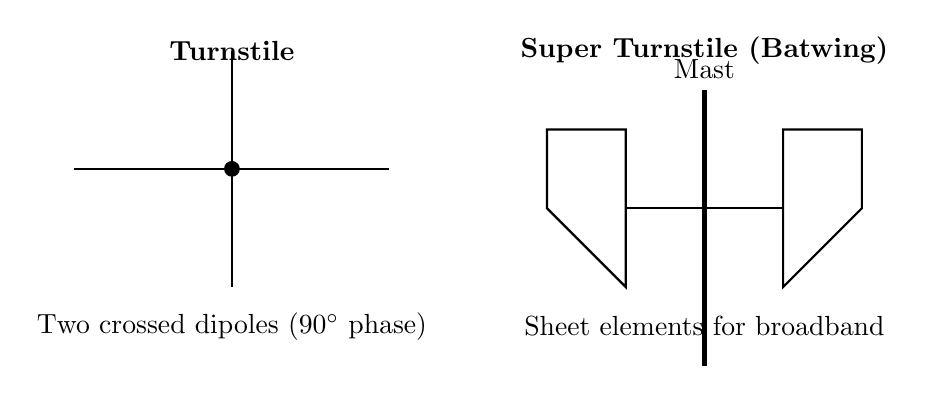
\begin{tikzpicture}
    % Turnstile
    \node [font=\bfseries] at (2, 3) {Turnstile};
    \draw [thick] (0, 1.5) -- (4, 1.5); % Horizontal 1
    \draw [thick] (2, 0) -- (2, 3);   % Horizontal 2 (Cross) - visual perspective
    \fill (2, 1.5) circle (0.1);
    \node at (2, -0.5) {Two crossed dipoles ($90^\circ$ phase)};
    
    % Super Turnstile (Batwing)
    \node [font=\bfseries] at (8, 3) {Super Turnstile (Batwing)};
    \draw [thick] (7, 0) -- (7, 2) -- (6, 2) -- (6, 1) -- cycle;
    \draw [thick] (9, 0) -- (9, 2) -- (10, 2) -- (10, 1) -- cycle;
    \draw [ultra thick] (8, -1) -- (8, 2.5) node [above] {Mast};
    \draw [thick] (7, 1) -- (9, 1); % Connection
    \node at (8, -0.5) {Sheet elements for broadband};
\end{tikzpicture}
\end{answerdiagram}

\begin{itemize}
    \item \textbf{Turnstile}: Provides omnidirectional horizontal pattern. Used in VHF/UHF.
    \item \textbf{Super Turnstile}: Broad bandwidth adaptation, commonly used in TV broadcasting.
\end{itemize}
\end{solutionbox}

\begin{mnemonicbox}
\mnemonic{"TACO: Turnstile Antennas Create Omnidirectional patterns"}
\end{mnemonicbox}

\orquestionmarks{4(b)}{4}{Give full form of MUF, LUF and OUF.}

\begin{solutionbox}
\begin{tabulary}{\linewidth}{|L|L|L|}
\hline
\textbf{Abbreviation} & \textbf{Full Form} & \textbf{Description} \\ \hline
\keyword{MUF} & Maximum Usable Frequency & The highest frequency that can be used for skywave communication between two specific points at a specific time. $f_{MUF} = f_c \sec \theta$. \\ \hline
\keyword{LUF} & Lowest Usable Frequency & The lowest frequency that provides satisfactory signal-to-noise ratio for a given circuit. Below this, absorption is too high. \\ \hline
\keyword{OUF (or OWF)} & Optimum Usable Frequency (Optimum Working Freq) & A frequency chosen for reliable communication, typically 85\% of the MUF to account for ionospheric variations. \\ \hline
\end{tabulary}

\begin{answerdiagram}{Frequency Selection}
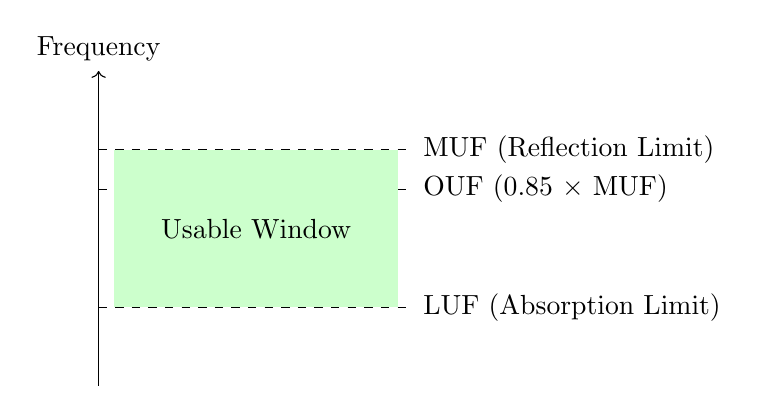
\begin{tikzpicture}
    \draw [->] (0,0) -- (0, 4) node [above] {Frequency};
    \draw [dashed] (0, 3) -- (4, 3) node [right] {MUF (Reflection Limit)};
    \draw [dashed] (0, 2.5) -- (4, 2.5) node [right] {OUF (0.85 $\times$ MUF)};
    \draw [dashed] (0, 1) -- (4, 1) node [right] {LUF (Absorption Limit)};
    
    \fill [green!20] (0.2, 1) rectangle (3.8, 3);
    \node at (2, 2) {Usable Window};
\end{tikzpicture}
\end{answerdiagram}
\end{solutionbox}

\begin{mnemonicbox}
\mnemonic{"MLO: Maximum and Lowest determine Optimum"}
\end{mnemonicbox}

\orquestionmarks{4(c)}{7}{Explain virtual height, critical frequency and skip distance in detail.}

\begin{solutionbox}
These are key parameters in skywave propagation via the ionosphere.

\begin{answerdiagram}{Ionospheric Reflection Parameters}
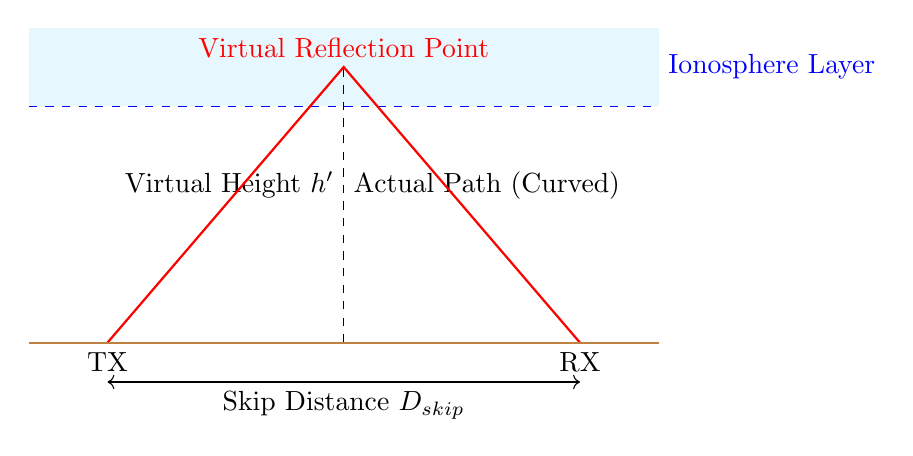
\begin{tikzpicture}
    % Ionosphere
    \fill [cyan!10] (-4, 3) rectangle (4, 4);
    \draw [dashed, blue] (-4, 3) -- (4, 3);
    \node [right, blue] at (4, 3.5) {Ionosphere Layer};
    
    % Virtual Height
    \draw [dashed] (0, 0) -- (0, 3.5);
    \node [right] at (0, 2) {Actual Path (Curved)};
    \node [left] at (0, 2) {Virtual Height $h'$};
    \draw [red, thick] (-3, 0) -- (0, 3.5) -- (3, 0); % Straight lines
    \node [red, above] at (0, 3.5) {Virtual Reflection Point};

    % Ground
    \draw [brown, thick] (-4, 0) -- (4, 0);
    \node [below] at (-3, 0) {TX};
    \node [below] at (3, 0) {RX};

    % Skip Distance
    \draw [<->] (-3, -0.5) -- (3, -0.5) node [midway, below] {Skip Distance $D_{skip}$};
\end{tikzpicture}
\end{answerdiagram}

\begin{enumerate}
    \item \textbf{Virtual Height ($h'$)}: The apparent height of the ionized layer as determined from the time interval between the transmitted pulse and the ionospheric echo at vertical incidence, assuming the wave travels at the speed of light $c$.
    
    \item \textbf{Critical Frequency ($f_c$)}: The highest frequency that is returned to earth by a layer when the wave is transmitted vertically ($\theta_i = 0$).
    $$ f_c = 9\sqrt{N_{max}} $$
    where $N_{max}$ is maximum electron density.
    
    \item \textbf{Skip Distance ($D_{skip}$)}: The minimum distance from the transmitter at which a sky wave of a given frequency (greater than $f_c$) can be returned to earth.
    $$ D_{skip} = 2h \sqrt{\left(\frac{f}{f_c}\right)^2 - 1} $$
    Or via secant law: $D = 2h \tan(\cos^{-1}(f_c/f))$.
\end{enumerate}
\end{solutionbox}

\begin{mnemonicbox}
\mnemonic{"VCS: Virtual height Controls Skip distance"}
\end{mnemonicbox}

\questionmarks{5(a)}{3}{With neat figure show different Ionosphere layers.}

\begin{solutionbox}
\begin{answerdiagram}{Ionospheric Layers}
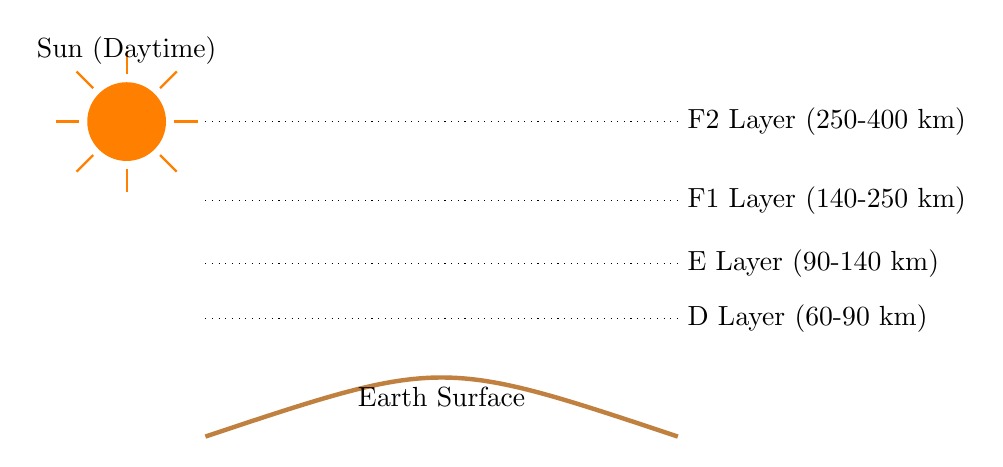
\begin{tikzpicture}
    % Earth
    \draw [ultra thick, brown] (-3, -1) .. controls (0, 0) .. (3, -1);
    \node at (0, -0.5) {Earth Surface};

    % Layers
    \draw [dotted] (-3, 0.5) -- (3, 0.5);
    \node [right] at (3, 0.5) {D Layer (60-90 km)};
    \draw [dotted] (-3, 1.2) -- (3, 1.2);
    \node [right] at (3, 1.2) {E Layer (90-140 km)};
    \draw [dotted] (-3, 2.0) -- (3, 2.0);
    \node [right] at (3, 2.0) {F1 Layer (140-250 km)};
    \draw [dotted] (-3, 3.0) -- (3, 3.0);
    \node [right] at (3, 3.0) {F2 Layer (250-400 km)};
    
    % Sun
    \fill [orange] (-4, 3) circle (0.5);
    \foreach \angle in {0, 45, ..., 360} \draw [thick, orange] (-4,3) ++(\angle:0.6) -- ++(\angle:0.3);
    \node [above] at (-4, 3.6) {Sun (Daytime)};
\end{tikzpicture}
\end{answerdiagram}

\begin{itemize}
    \item \textbf{D Layer}: Absorbs HF waves, disappears at night.
    \item \textbf{E Layer}: Reflects some HF waves, sporadic E.
    \item \textbf{F1/F2 Layers}: Main reflecting layers for long-distance skywave communication. F1/F2 merge at night.
\end{itemize}
\end{solutionbox}

\begin{mnemonicbox}
\mnemonic{"DEAF: Down to up - D, E, And F layers"}
\end{mnemonicbox}

\questionmarks{5(b)}{4}{Give names of different types of satellite communication systems and compare it.}

\begin{solutionbox}
\begin{tabulary}{\linewidth}{|L|L|L|}
\hline
\textbf{System} & \textbf{Orbit} & \textbf{Characteristics} \\ \hline
\keyword{GEO (Geostationary)} & 35,786 km (Equatorial) & Stationary relative to earth. High latency ($\sim$240ms). Wide coverage (3 sats for global). TV, Weather. \\ \hline
\keyword{MEO (Medium Earth)} & 2,000 - 35,000 km & Lower latency than GEO. Used for GPS, GLONASS. \\ \hline
\keyword{LEO (Low Earth)} & 160 - 2,000 km & Low latency ($\sim$20ms). Moving fast relative to earth. Requires constellation for coverage. Iridium, Starlink. \\ \hline
\keyword{HEO (Highly Elliptical)} & Elliptical & Molniya orbit. High dwell time over high latitudes (Polar regions). \\ \hline
\end{tabulary}

\begin{answerdiagram}{Orbit Comparison}
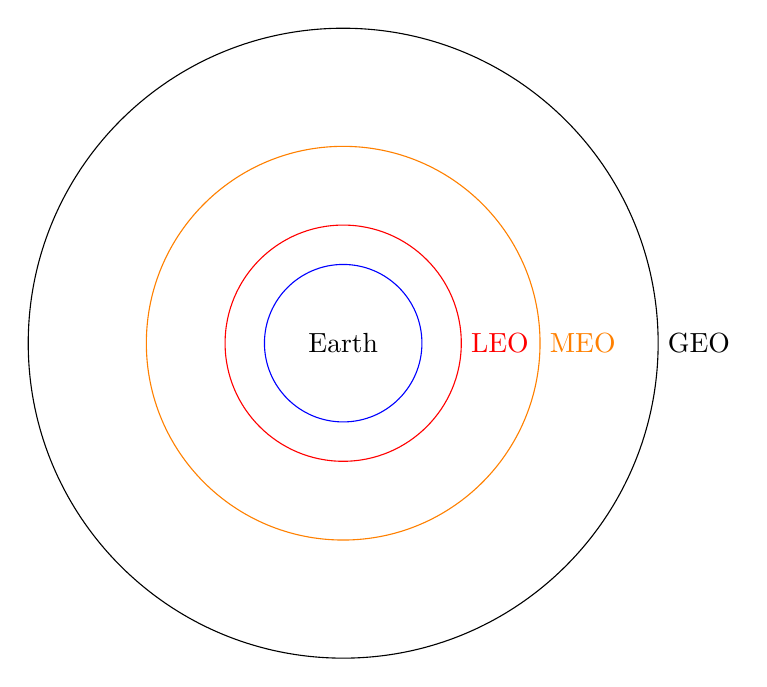
\begin{tikzpicture}
    \draw [blue] (0,0) circle (1); \node at (0,0) {Earth};
    \draw [red] (0,0) circle (1.5); \node [red, right] at (1.5, 0) {LEO};
    \draw [orange] (0,0) circle (2.5); \node [orange, right] at (2.5, 0) {MEO};
    \draw [black] (0,0) circle (4); \node [black, right] at (4, 0) {GEO};
\end{tikzpicture}
\end{answerdiagram}
\end{solutionbox}

\begin{mnemonicbox}
\mnemonic{"TBDMN: Telecom, Broadcasting, Data, Military, Navigation"}
\end{mnemonicbox}

\questionmarks{5(c)}{7}{Draw and explain DTH receiver system.}

\begin{solutionbox}
\textbf{DTH (Direct-To-Home)}: A satellite television broadcasting system where TV programs are transmitted directly to the subscriber's premises using Ku-band satellites.

\begin{answerdiagram}{DTH System Block Diagram}
\begin{tikzpicture}[node distance=1.5cm, auto]
    % Satellite
    \node (sat) at (0, 3) [cloud, draw, aspect=2, blue] {Satellite (Ku-Band)};
    
    % Dish
    \node (dish) at (0, 1) [draw, semicircle, rotate=90, minimum width=1cm] {}; 
    \draw [thick] (dish.south) -- ++(0.5, 0); 
    \node [left] at (-0.5, 1) {Dish + LNB};
    
    % Blocks
    \node [gtu block, below=of dish] (stb) {Set-Top Box (STB)};
    \node [gtu block, below=of stb] (tv) {TV Set};

    \draw [gtu arrow, dashed] (sat) -- node [right] {Signal (10-12 GHz)} (dish);
    \draw [gtu arrow] (dish) -- node [right] {Coax (IF 950-2150 MHz)} (stb);
    \draw [gtu arrow] (stb) -- node [right] {Audio/Video} (tv);
\end{tikzpicture}
\end{answerdiagram}

\textbf{Components}:
\begin{enumerate}
    \item \textbf{Parabolic Dish}: 60-90 cm offset dish to collect weak satellite signals.
    \item \textbf{LNBF (Low Noise Block Feedhorn)}: Amplifies the weak Ku-band signal and downconverts it to IF (Intermediate Frequency) range for transmission over cable.
    \item \textbf{Coaxial Cable}: RG-6 cable transmits IF signal to STB.
    \item \textbf{Set-Top Box (STB)}: Contains tuner, demodulator (QPSK/8PSK), and decoder (MPEG-2/4) to convert digital signals into video/audio for TV.
    \item \textbf{Smart Card}: For conditional access (decrypting paid channels).
\end{enumerate}
\end{solutionbox}

\begin{mnemonicbox}
\mnemonic{"DOCS: Dish Obtains, Converts and Shows signals"}
\end{mnemonicbox}

\orquestionmarks{5(a)}{3}{What is the Need of Smart Antennas? Write its applications.}

\begin{solutionbox}
\textbf{Smart Antenna}: An array of antennas with smart signal processing algorithms used to identify spatial signal signatures and calculate beamforming vectors to track the desired user.

\textbf{Need}:
\begin{itemize}
    \item \textbf{Capacity Increase}: Allows spatial division multiple access (SDMA), serving more users.
    \item \textbf{Range Extension}: High directive gain extends cell coverage.
    \item \textbf{Interference Rejection}: Nulls can be steered towards interferers.
    \item \textbf{Power Efficiency}: Directs energy only where needed.
\end{itemize}

\textbf{Applications}:
\begin{itemize}
    \item 4G/5G Cellular Networks (MIMO).
    \item Radar Systems.
    \item Wi-Fi (Beamforming routers).
    \item Satellite Communications.
\end{itemize}
\end{solutionbox}

\begin{mnemonicbox}
\mnemonic{"SAFE: Smart Antennas For Efficiency"}
\end{mnemonicbox}

\orquestionmarks{5(b)}{4}{Explain Kepler's 3rd law.}

\begin{solutionbox}
\textbf{Kepler's 3rd Law (Law of Periods)}:
The square of the orbital period ($T$) of a planet or satellite is directly proportional to the cube of the semi-major axis ($a$) of its orbit.

$$ T^2 \propto a^3 $$
$$ T^2 = \left( \frac{4\pi^2}{GM} \right) a^3 $$

Where:
\begin{itemize}
    \item $T$: Orbital period (seconds)
    \item $a$: Semi-major axis (meters) - radius for circular orbit.
    \item $G$: Gravitational constant ($6.67 \times 10^{-11} Nm^2/kg^2$)
    \item $M$: Mass of the central body (Earth).
\end{itemize}

\begin{answerdiagram}{Kepler's 3rd Law}
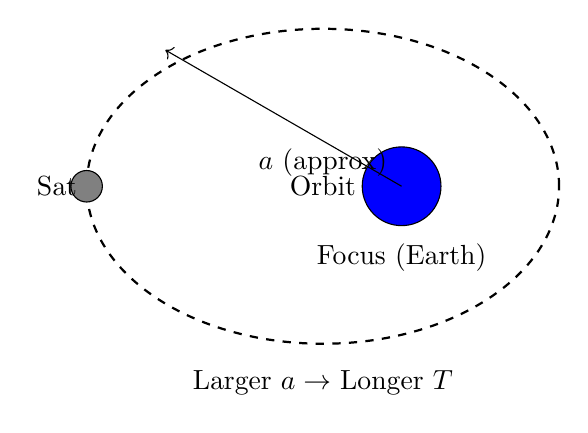
\begin{tikzpicture}
    \draw [thick, dashed] (0,0) ellipse (3 and 2);
    \draw [fill=blue] (1,0) circle (0.5); \node [below] at (1, -0.6) {Focus (Earth)};
    \draw [fill=gray] (-3, 0) circle (0.2); \node [left] at (-3, 0) {Sat};
    
    \draw [->] (1,0) -- (-2, 1.73); \node [midway, above] {$a$ (approx)};
    \node at (0, 0) {Orbit};
    \node at (0, -2.5) {Larger $a \rightarrow$ Longer $T$};
\end{tikzpicture}
\end{answerdiagram}
\end{solutionbox}

\begin{mnemonicbox}
\mnemonic{"CAP: Cube of Axis equals Period squared"}
\end{mnemonicbox}

\orquestionmarks{5(c)}{7}{Identify the different types of Antennas for Terrestrial Mobile communication and explain in detail.}

\begin{solutionbox}
Detailed explanation of Base Station and Mobile Station antennas.

\begin{tabulary}{\linewidth}{|L|L|L|}
\hline
\textbf{Type} & \textbf{Example} & \textbf{Feature} \\ \hline
\keyword{Base Station} & Sectoral Panels & Directional ($120^\circ$), High Gain, Vertical Array. \\ \hline
\keyword{Mobile Station} & PIFA, Monopole & Omnidirectional, Compact, Multi-band. \\ \hline
\keyword{MIMO} & Multiple Elements & Spatial diversity, Multiplexing. \\ \hline
\end{tabulary}

\begin{answerdiagram}{Base Station Sector Antenna}
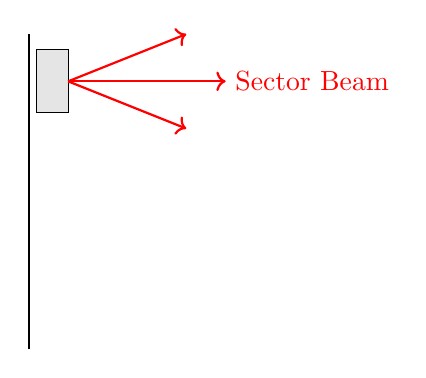
\begin{tikzpicture}
    % Tower
    \draw [thick] (0,0) -- (0, 4);
    % Panel
    \draw [fill=gray!20] (0.1, 3) rectangle (0.5, 3.8);
    % Radiation
    \draw [->, red, thick] (0.5, 3.4) -- (2, 4);
    \draw [->, red, thick] (0.5, 3.4) -- (2.5, 3.4);
    \draw [->, red, thick] (0.5, 3.4) -- (2, 2.8);
    \node [right, red] at (2.5, 3.4) {Sector Beam};
\end{tikzpicture}
\end{answerdiagram}

\textbf{Explanation}:
\begin{enumerate}
    \item \textbf{Base Station Antennas}:
    \begin{itemize}
        \item Typically Collinear Dipole Arrays inside a radome.
        \item Used to cover a specific sector (e.g., 3 sectors of 120 degrees each).
        \item Provide high gain in horizontal direction and narrow beam vertical direction.
        \item Supports electrical or mechanical downtilt to contain coverage.
    \end{itemize}
    \item \textbf{Mobile Antennas}:
    \begin{itemize}
        \item \textbf{PIFA (Planar Inverted-F Antenna)}: Very common in phones. Compact, built onto PCB.
        \item \textbf{Monopole/Whip}: Used on vehicles.
        \item Features: Omnidirectional in azimuth plane to allow reception from any direction.
    \end{itemize}
\end{enumerate}
\end{solutionbox}

\begin{mnemonicbox}
\mnemonic{"BEST: Base-stations Employ Sector Technology"}
\end{mnemonicbox}

\end{document}
